\section{Continuous Regression Modeling}
\label{sec:activity1-continuous-regression}

Continuous regression addresses the predictive component of Research Question 1:
how accurately can salary be predicted, and which factors drive income. Five
candidate models are constructed on a common training set. All five models use
$\ln(\mathrm{salary})$ as the response: full and stepwise
multiple linear regression, ridge regression, LASSO
regression, and elastic-net regression. A sixth model uses the Box--Cox response
$\mathrm{salary}^{0.26}$ selected in \cref{subsec:multiple-linear-regression}.
\Cref{tab:model-overview} summarizes these models.

An untransformed salary model is also fitted as a diagnostic baseline for the
Box--Cox analysis and response-scale comparison, but it is not a candidate for the
final comparison. The log response is retained as the primary specification for
inference because its coefficients can be interpreted as percentage effects. All
models are compared on a held-out test set, and the model selection and
recommendation are presented in \cref{sec:activity1-model-evaluation}.

All models use the same reference categories - the category to which every
other level of a factor is compared - for the five categorical predictors: Entry
for experience, Full-time for employment type, Data\_Analyst for job
category, Small for company size, and Rest-of-world for location. Every
specification also includes the binary \texttt{is\_local} indicator which was
introduced in \cref{sec:activity1-data-preprocessing} as a low-collinearity
alternative to the near-redundant employee-residence dummies.

\begin{table}[htbp]
    \centering
    \caption{Candidate regression models and their fitted response scales.}
    \label{tab:model-overview}
    \small
    \begin{tabular}{ll}
        \toprule
        \textbf{Model} & \textbf{Fitted response} \\
        \midrule
        Multiple linear regression (full)     & $\ln(\mathrm{salary})$ \\
        Multiple linear regression (stepwise) & $\ln(\mathrm{salary})$ \\
        Ridge regression                      & $\ln(\mathrm{salary})$ \\
        LASSO regression                      & $\ln(\mathrm{salary})$ \\
        Elastic-net regression                & $\ln(\mathrm{salary})$ \\
        Box--Cox power regression             & $\mathrm{salary}^{0.26}$ \\
        \bottomrule
    \end{tabular}
\end{table}

\subsection{Train/Test Split}
\label{subsec:train-test-split}

A plain random 80:20 split partitions the 565 observations into a training set of
452 and a test set of 113. The random seed is set with
\texttt{set.seed(2026)} to ensure reproducibility. This simple random split is
appropriate because the research question concerns global salary prediction across
all years rather than forecasting a specific future year. The split is constrained
so that every level of the five categorical predictors (experience, employment
type, job category, company size, location) observed in the test set is also
represented in the training set, preventing factor-based models from encountering
unseen levels during prediction. Model fitting, tuning, and cross-validation are
performed exclusively on the training set, as described in this section. The
untouched test set is used only once for the governed evaluation in
\cref{sec:activity1-model-evaluation}. Its composition is reported in
\cref{tab:train-test-split}.

\begin{table}[htbp]
    \centering
    \caption{Train/test composition by work year.}
    \label{tab:train-test-split}
    \small
    \begin{tabular}{lccc}
        \toprule
        \textbf{Work year} & \textbf{Train} & \textbf{Test} & \textbf{Total} \\
        \midrule
        2020  & 58  & 14  & 72  \\
        2021  & 172 & 43  & 215 \\
        2022  & 222 & 56  & 278 \\
        \midrule
        Total & 452 & 113 & 565 \\
        \bottomrule
    \end{tabular}
\end{table}

\subsection{Multiple Linear Regression}
\label{subsec:multiple-linear-regression}

The initial model applies ordinary least squares to untransformed salary,
\[
    \mathrm{salary} = \alpha + X\beta + \varepsilon,
\]
using the full predictor set on the training data, where it explains 47.6\% of the
variance ($R^2_{\mathrm{adj}} = 0.462$). The residual diagnostics nevertheless
warrant a response transformation on other grounds: the Shapiro--Wilk test rejects
residual normality ($p \approx 1.3 \times 10^{-21}$) and the maximum Cook's distance
is 0.180. Once \texttt{is\_local} is controlled, the Breusch--Pagan test flags
unequal variances ($\chi^2 = 41.6$, $p = 0.010$); the case for transformation
rests on the strong right skew identified in \cref{sec:activity1-eda}, the
severe non-normality, and heteroskedasticity.

\begin{figure}[htbp]
    \centering
    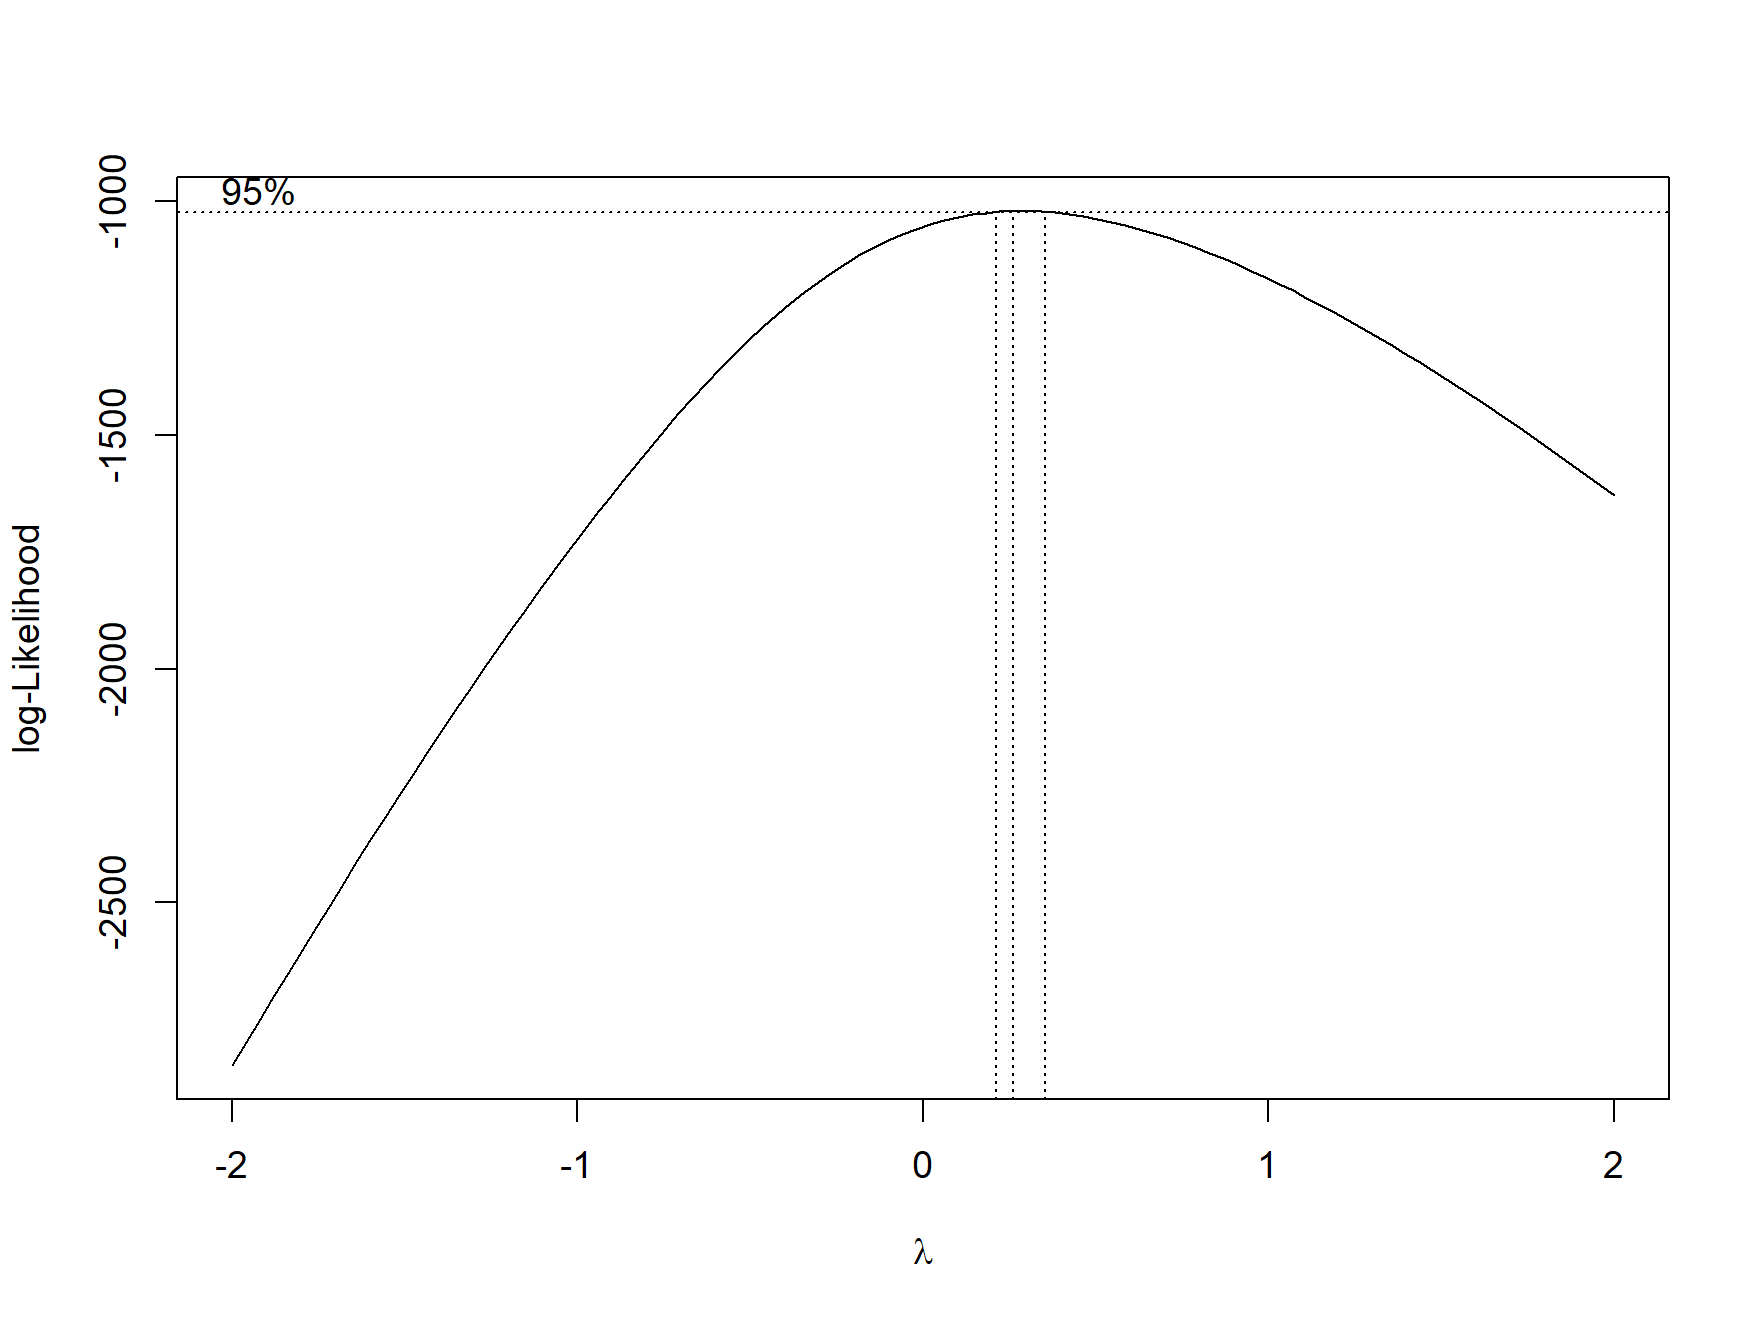
\includegraphics[width=0.75\textwidth]{img/activity1/06_boxcox.png}
    \caption{Box--Cox likelihood profile for the raw-salary model. The likelihood is
    maximized near $\hat{\lambda}=0.26$. The dotted horizontal line denotes the 95\%
    profile-likelihood cutoff.}
    \label{fig:boxcox-profile}
\end{figure}

The Box--Cox profile in \cref{fig:boxcox-profile} peaks at
$\hat{\lambda} \approx 0.26$, with a 95\% profile-likelihood interval $[0.22,\ 0.34]$
that excludes both the identity transformation ($\lambda=1$) and the logarithmic
transformation ($\lambda=0$), indicating that the likelihood favors the intermediate
response $\mathrm{salary}^{0.26}$. Nevertheless,
$\ln(\mathrm{salary})$ is retained as the primary inferential response because its
coefficients have direct percentage interpretations. The Box--Cox model remains a
candidate for prediction.

The Box--Cox family transforms the raw response as
\[
    y^{(\lambda)} =
    \begin{cases}
        \dfrac{y^{\lambda} - 1}{\lambda}, & \lambda \neq 0,\\[1.4ex]
        \ln y,                             & \lambda = 0,
    \end{cases}
\]
and $\lambda$ is estimated by profile likelihood on the training set, giving
$\hat{\lambda} \approx 0.26$ and hence the power response
$\mathrm{salary}^{0.26}$.

\Cref{tab:response-scale-diagnostics} compares the raw, Box--Cox, and log response
scales using the same predictors. No transformation fully resolves the diagnostic
violations---residual normality is rejected on every scale. The Box--Cox model has
the highest adjusted $R^2$ (0.623) and the smallest maximum Cook's distance (0.048),
whereas the log response has slightly lower adjusted $R^2$ (0.619) and the raw scale
shows the strongest heteroskedasticity.

\begin{table}[htbp]
    \centering
    \caption{Training-set residual diagnostics under alternative response scales.}
    \label{tab:response-scale-diagnostics}
    \small
    \begin{tabular}{lccccc}
        \toprule
        \textbf{Response}
            & \textbf{Shapiro--Wilk} $p$
            & \textbf{BP} $\chi^2$
            & \textbf{BP} $p$
            & \textbf{Max Cook's} $D$
            & $R^2_{\mathrm{adj}}$ \\
        \midrule
        $\mathrm{salary}$
            & $1.3 \times 10^{-21}$ & 41.6 & 0.010    & 0.180 & 0.462 \\
        $\mathrm{salary}^{0.26}$
            & $1.8 \times 10^{-9}$  & 34.6 & 0.057    & 0.048 & 0.623 \\
        $\ln(\mathrm{salary})$
            & $1.9 \times 10^{-14}$ & 40.9 & 0.012    & 0.048 & 0.619 \\
        \bottomrule
    \end{tabular}
\end{table}

\paragraph{Log-scale model.}
The full log-scale model achieves $R^2_{\mathrm{adj}}=0.619$
($F_{23,428}=32.8$, $p<10^{-16}$). Generalized variance inflation factors range from
about 1.03 to 1.26 (including 1.06 for \texttt{is\_local}), indicating negligible
multicollinearity. Residual normality is still rejected, although the
Shapiro--Wilk $p$-value rises from approximately $1.3 \times 10^{-21}$ to
$1.9 \times 10^{-14}$ --- a roughly 14-million-fold improvement. The maximum
Cook's distance decreases from 0.180 to 0.048, while heteroskedasticity remains
present under the log response ($\chi^2=40.9$, $p=0.012$).

Stepwise selection by AIC trims the full log model (AIC 676.4) to a reduced model
(AIC 673.5) by removing only \texttt{work\_year} and \texttt{remote\_ratio}, at
essentially unchanged adjusted $R^2$ (0.619 vs 0.620); both terms are removed.
Thus the data provide little evidence of a separate linear effect of
remote ratio and work year after adjustment for location, experience, and job
category. HC1 robust standard errors preserve all substantive conclusions.
Notably, the medium-company contrast is significant under both conventional
and robust inference ($p=0.010$ conventional; $p=0.048$ robust), so both
medium and large company contrasts are treated as reliable.

\paragraph{Estimated salary drivers.}
For a log-response model, the percentage effect of a coefficient is calculated as
$100(e^{\hat{\beta}}-1)\%$. The estimates from the stepwise model, together with
their significance, are collected in \cref{tab:driver-effects}. The substantive
interpretation of these coefficient magnitudes, and which factors most strongly
drive income, is discussed in \cref{sec:activity1-feature-importance}.

\begin{table}[htbp]
    \centering
    \caption{Estimated percentage effects from the stepwise log-scale model.}
    \label{tab:driver-effects}
    \small
    \begin{tabular}{llcc}
        \toprule
        \textbf{Factor} & \textbf{Contrast (vs. baseline)}
            & \textbf{Effect} & \textbf{Significance} \\
        \midrule
        Experience (vs. Entry)
            & Mid       & +24\%  & *** \\
            & Senior    & +68\%  & *** \\
            & Executive & +159\% & *** \\
        \addlinespace[0.35em]
        Job category (vs. Data Analyst)
            & Engineer          & +31\% & ***  \\
            & Data Scientist    & +35\% & *** \\
            & ML/AI Engineer    & +46\% & *** \\
            & Management / Lead & +54\% & *** \\
            & Research          & +62\% & *** \\
            & Other             & +9\%  & n.s. \\
        \addlinespace[0.35em]
        Employment type (vs. Full-time)
            & Contract  & +30\%   & n.s. \\
            & Part-time & $-69\%$ & *** \\
            & Freelance & $-73\%$ & *** \\
        \addlinespace[0.35em]
        Company size (vs. Small)
            & Medium & +21\% & ** \\
            & Large  & +37\% & *** \\
        \addlinespace[0.35em]
        Location (vs. Rest-of-world)
            & India         & $-48\%$ & *** \\
            & Spain         & $-5\%$  & n.s. \\
            & France        & +40\%   & *   \\
            & Germany       & +77\%   & *** \\
            & Great Britain & +73\%   & *** \\
            & Canada        & +98\%   & *** \\
            & United States & +162\%  & *** \\
        \addlinespace[0.35em]
        Local employment (vs. foreign)
            & \texttt{is\_local} & +46\% & *** \\
        \bottomrule
    \end{tabular}

    \vspace{0.4em}
    \begin{minipage}{0.92\textwidth}
        \footnotesize
        Significance codes: *** $p<0.001$, ** $p<0.01$, * $p<0.05$;
        n.s. denotes non-significance at the 5\% level.
    \end{minipage}
\end{table}

\subsection{Ridge, LASSO, and Elastic-Net Regression}
\label{subsec:regularized-regression}

Regularized regression introduces bias to reduce estimation variance and provides an
independent assessment of the stepwise variable selection. Four numeric inputs
(\texttt{exp\_level\_ord}, \texttt{company\_size\_ord},
\texttt{remote\_ratio}, and \texttt{work\_year}) were standardized using
training-set means and standard deviations and enter as continuous predictors. These
were combined with the dummy variables for job category, employment type, and
location together with the binary \texttt{is\_local} indicator (which, being a 0/1
indicator, needs no scaling), producing 21 predictors.

The penalty parameter $\lambda$ was selected by ten-fold cross-validation within the
training set. Predictions use $\lambda_{\min}$, while $\lambda_{1se}$ is reported as
a more strongly regularized alternative. The ridge and LASSO cross-validation paths
are shown in \cref{fig:cv-curves}.

\begin{figure}[htbp]
    \centering
    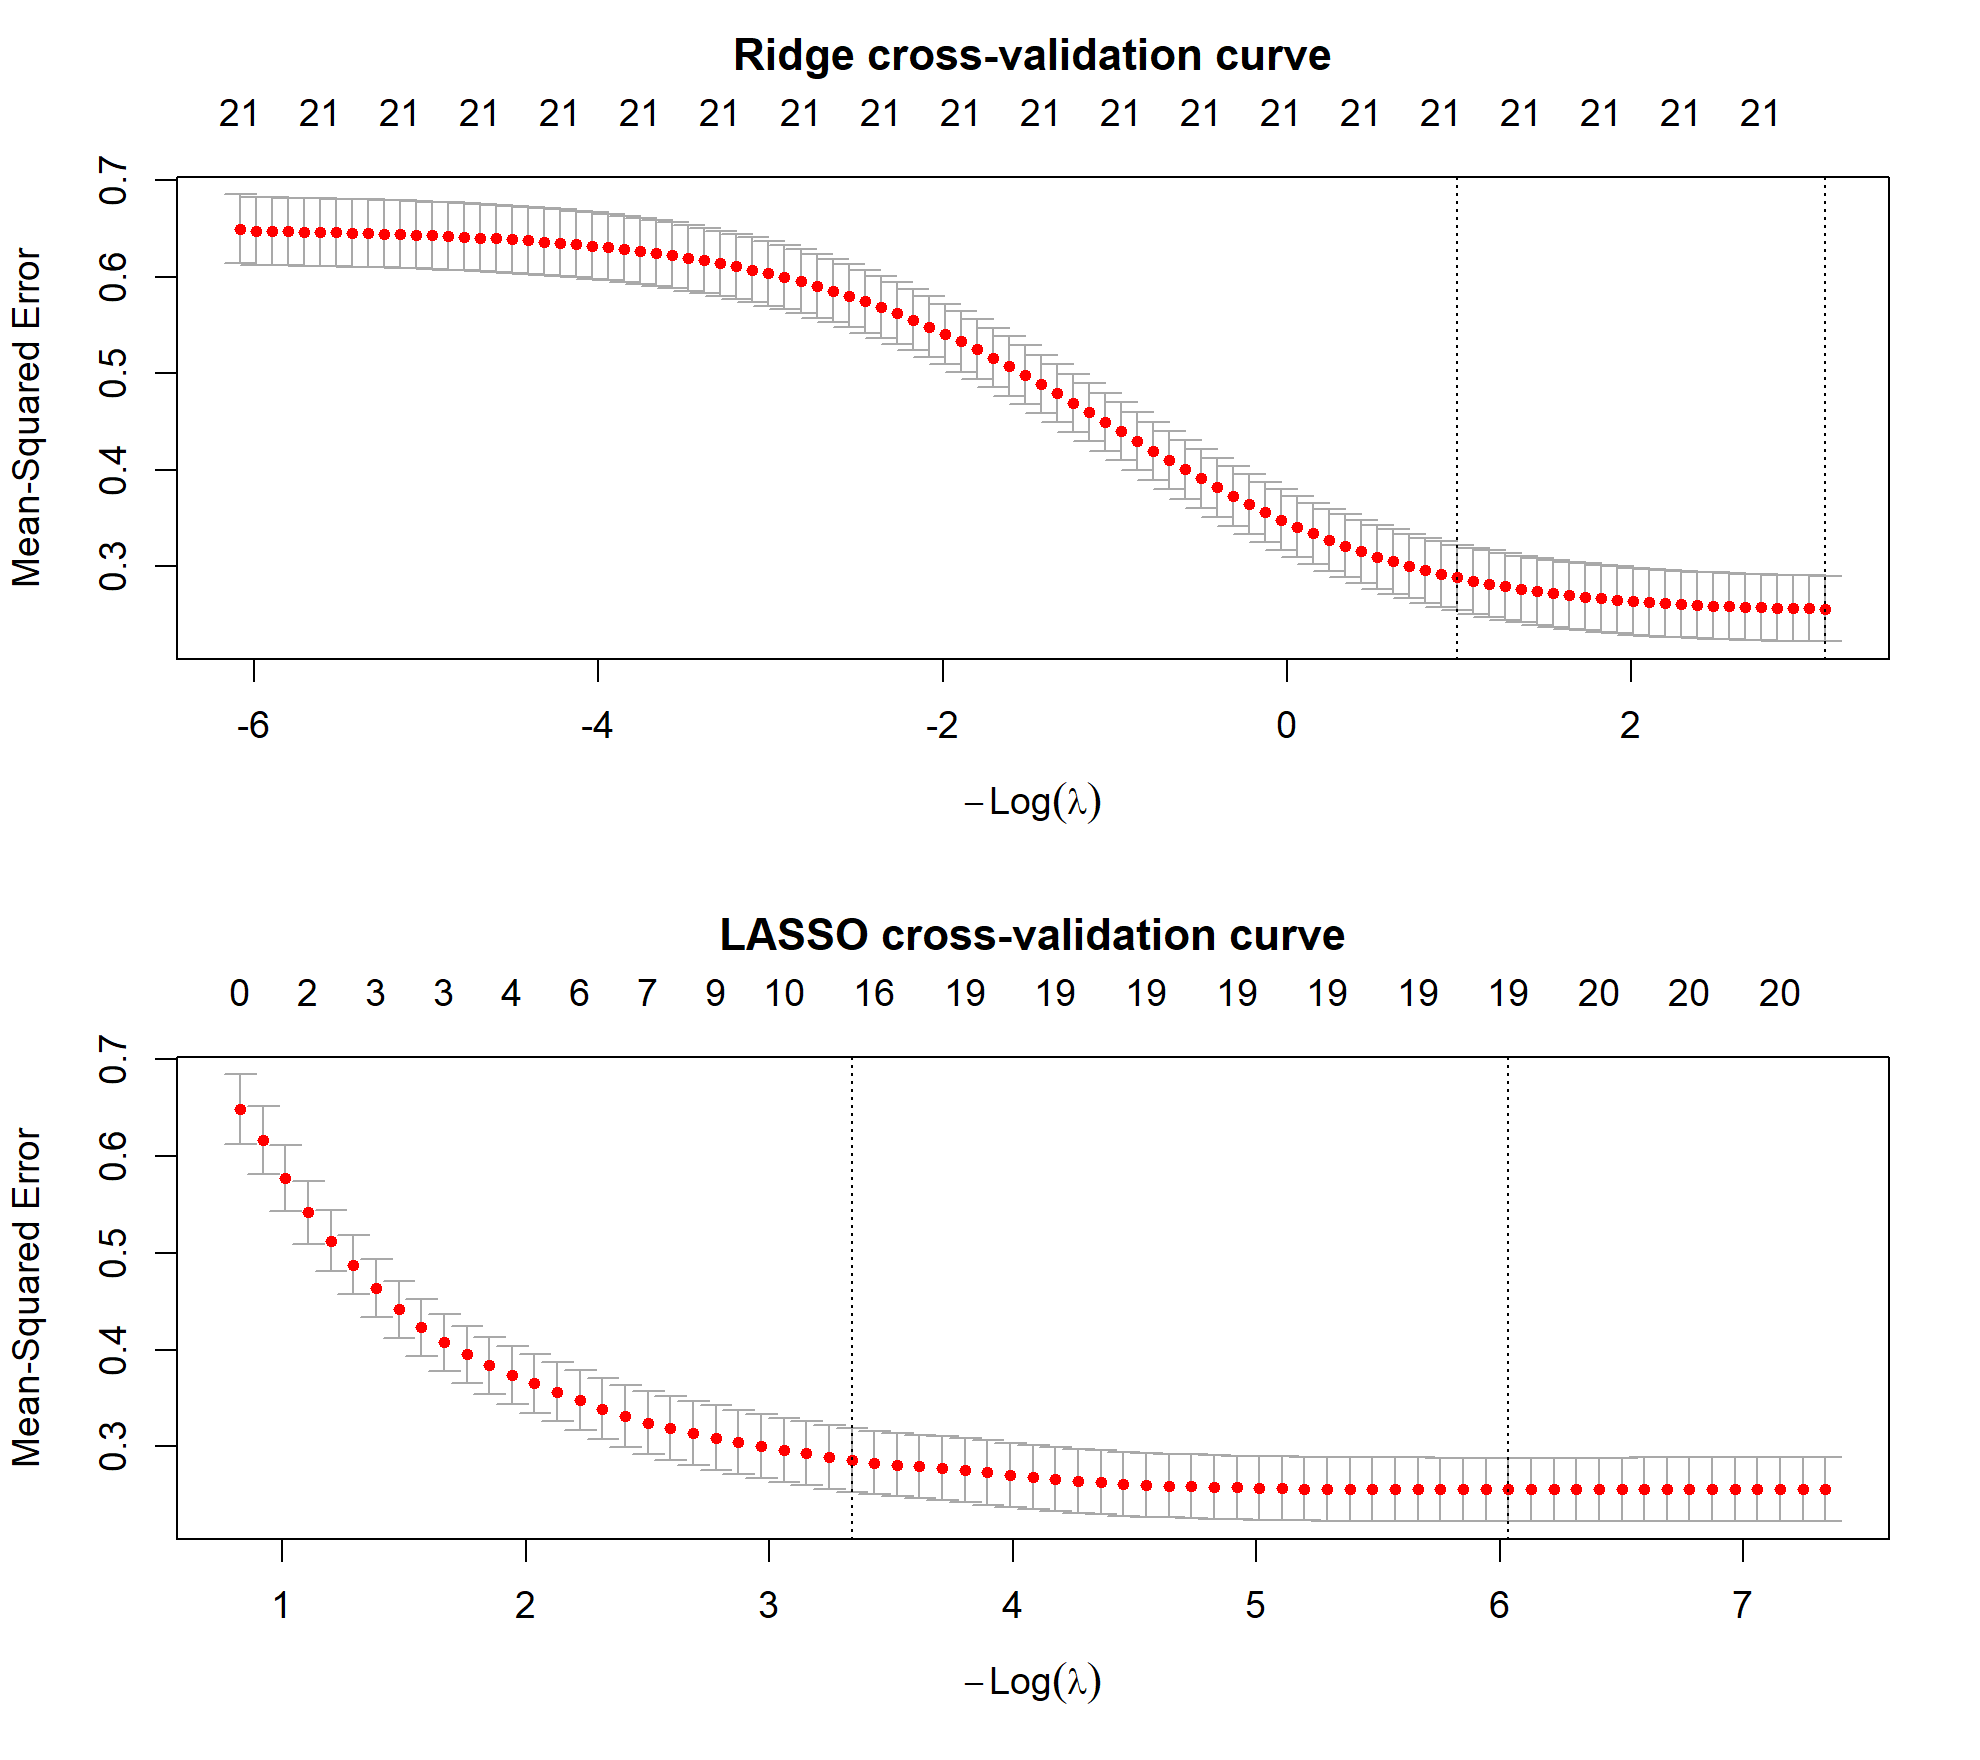
\includegraphics[width=0.85\textwidth]{img/activity1/06_ridge_lasso_cv.png}
    \caption{Ten-fold cross-validation curves for ridge regression (top) and LASSO
    regression (bottom). Vertical dotted lines indicate $\lambda_{\min}$ and
    $\lambda_{1se}$; numbers above each panel denote the number of nonzero
    coefficients.}
    \label{fig:cv-curves}
\end{figure}

Ridge regression selects $\lambda_{\min}=0.0462$ and
$\lambda_{1se}=0.2969$. It shrinks the coefficients smoothly and generalizes better
than the full OLS model. LASSO selects
$\lambda_{\min}=6.25 \times 10^{-4}$ and retains all 21 predictors, providing no
evidence for a substantially sparser solution at $\lambda_{\min}$.

Both estimators minimize the penalized residual sum of squares
\[
    \hat{\beta} = \arg\min_{\beta} \left\{
        \sum_{i=1}^{n}\bigl(y_i - x_i^{\top}\beta\bigr)^2
        + \lambda\, P(\beta)
    \right\},
\]
where the penalty is the ridge $P(\beta) = \|\beta\|_2^2 = \sum_j \beta_j^2$ or
the LASSO $P(\beta) = \|\beta\|_1 = \sum_j |\beta_j|$.

\textbf{Elastic-net regression.} Ridge and LASSO are the two ends of a single
elastic-net family, whose penalty is a weighted mixture of the L2 (ridge) and L1
(LASSO) terms,
\[
    \lambda\bigl[\alpha\,\lVert\beta\rVert_1 + (1-\alpha)\,\lVert\beta\rVert_2^2\bigr],
\]
where $\alpha=0$ recovers pure ridge and $\alpha=1$ recovers pure LASSO; intermediate
values select the mixture between them. The mixing parameter $\alpha$ was tuned on the
same grid $\alpha=0,0.1,\ldots,1$ by ten-fold cross-validation within the training
set. As \cref{fig:enet-sweep} shows, the cross-validation error is almost flat across
the entire range, moving only from 0.5153 to 0.5161 (a difference of 0.0008 log
points, about 0.16\%). The selected value is $\alpha=0.1$, and because the
surface is so flat, predictive performance is insensitive to the penalty mixture over
the examined grid; all regularized models are therefore carried into the final
comparison.

\begin{figure}[htbp]
    \centering
    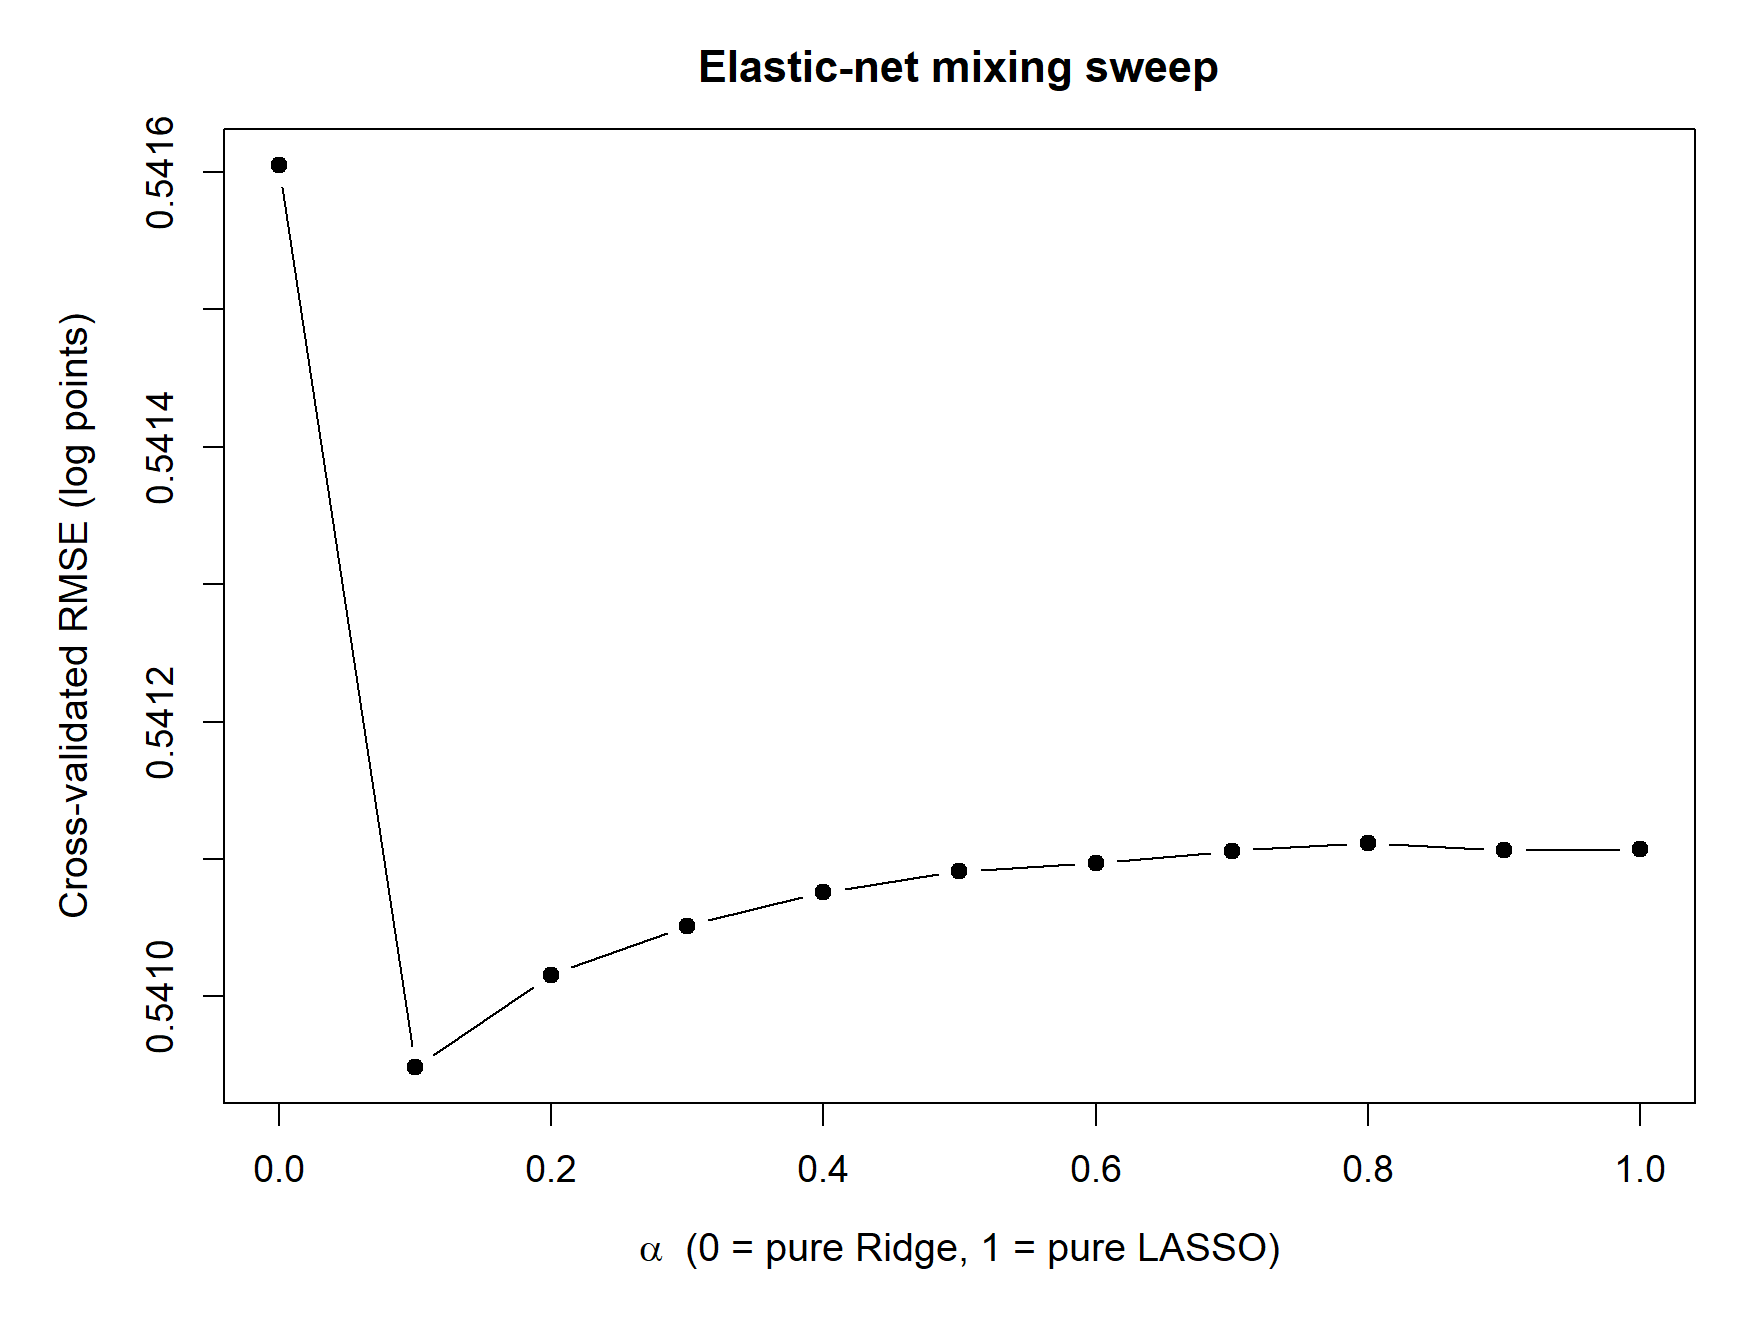
\includegraphics[width=0.75\linewidth]{img/activity1/06_enet_alpha_sweep.png}
    \caption{Cross-validated RMSE as a function of the elastic-net mixing parameter
    $\alpha$. The surface is nearly flat (0.5153--0.5161), indicating that the
    ridge--LASSO mixture has little effect on predictive accuracy; the minimum is at
    $\alpha=0.1$.}
    \label{fig:enet-sweep}
\end{figure}

Mapping dummy coefficients to their parent variables also shows close agreement
between stepwise selection and LASSO. Both retain the substantive predictor blocks
---experience, job category, employment type, company size, and location (including
\texttt{is\_local})---and both keep a component for \texttt{remote\_ratio}. The only
difference is that LASSO retains a small linear component for \texttt{work\_year},
which the AIC-based procedure removes. Replacing the ordinal encodings of experience
and company size with full dummy encodings produces similar predictive performance
(cross-validated RMSE 0.5154 versus 0.5176).

This section has described how each candidate model was constructed and how its
assumptions were checked. All six candidate models are scored on a common held-out
test set and formally compared, with the model selection and recommendation,
in \cref{sec:activity1-model-evaluation}.